\section{Geometric modelling and transformations}
\label{sec:objects_modelling}
\begin{figure}[H]\centering
\begin{minipage}{0.49\linewidth}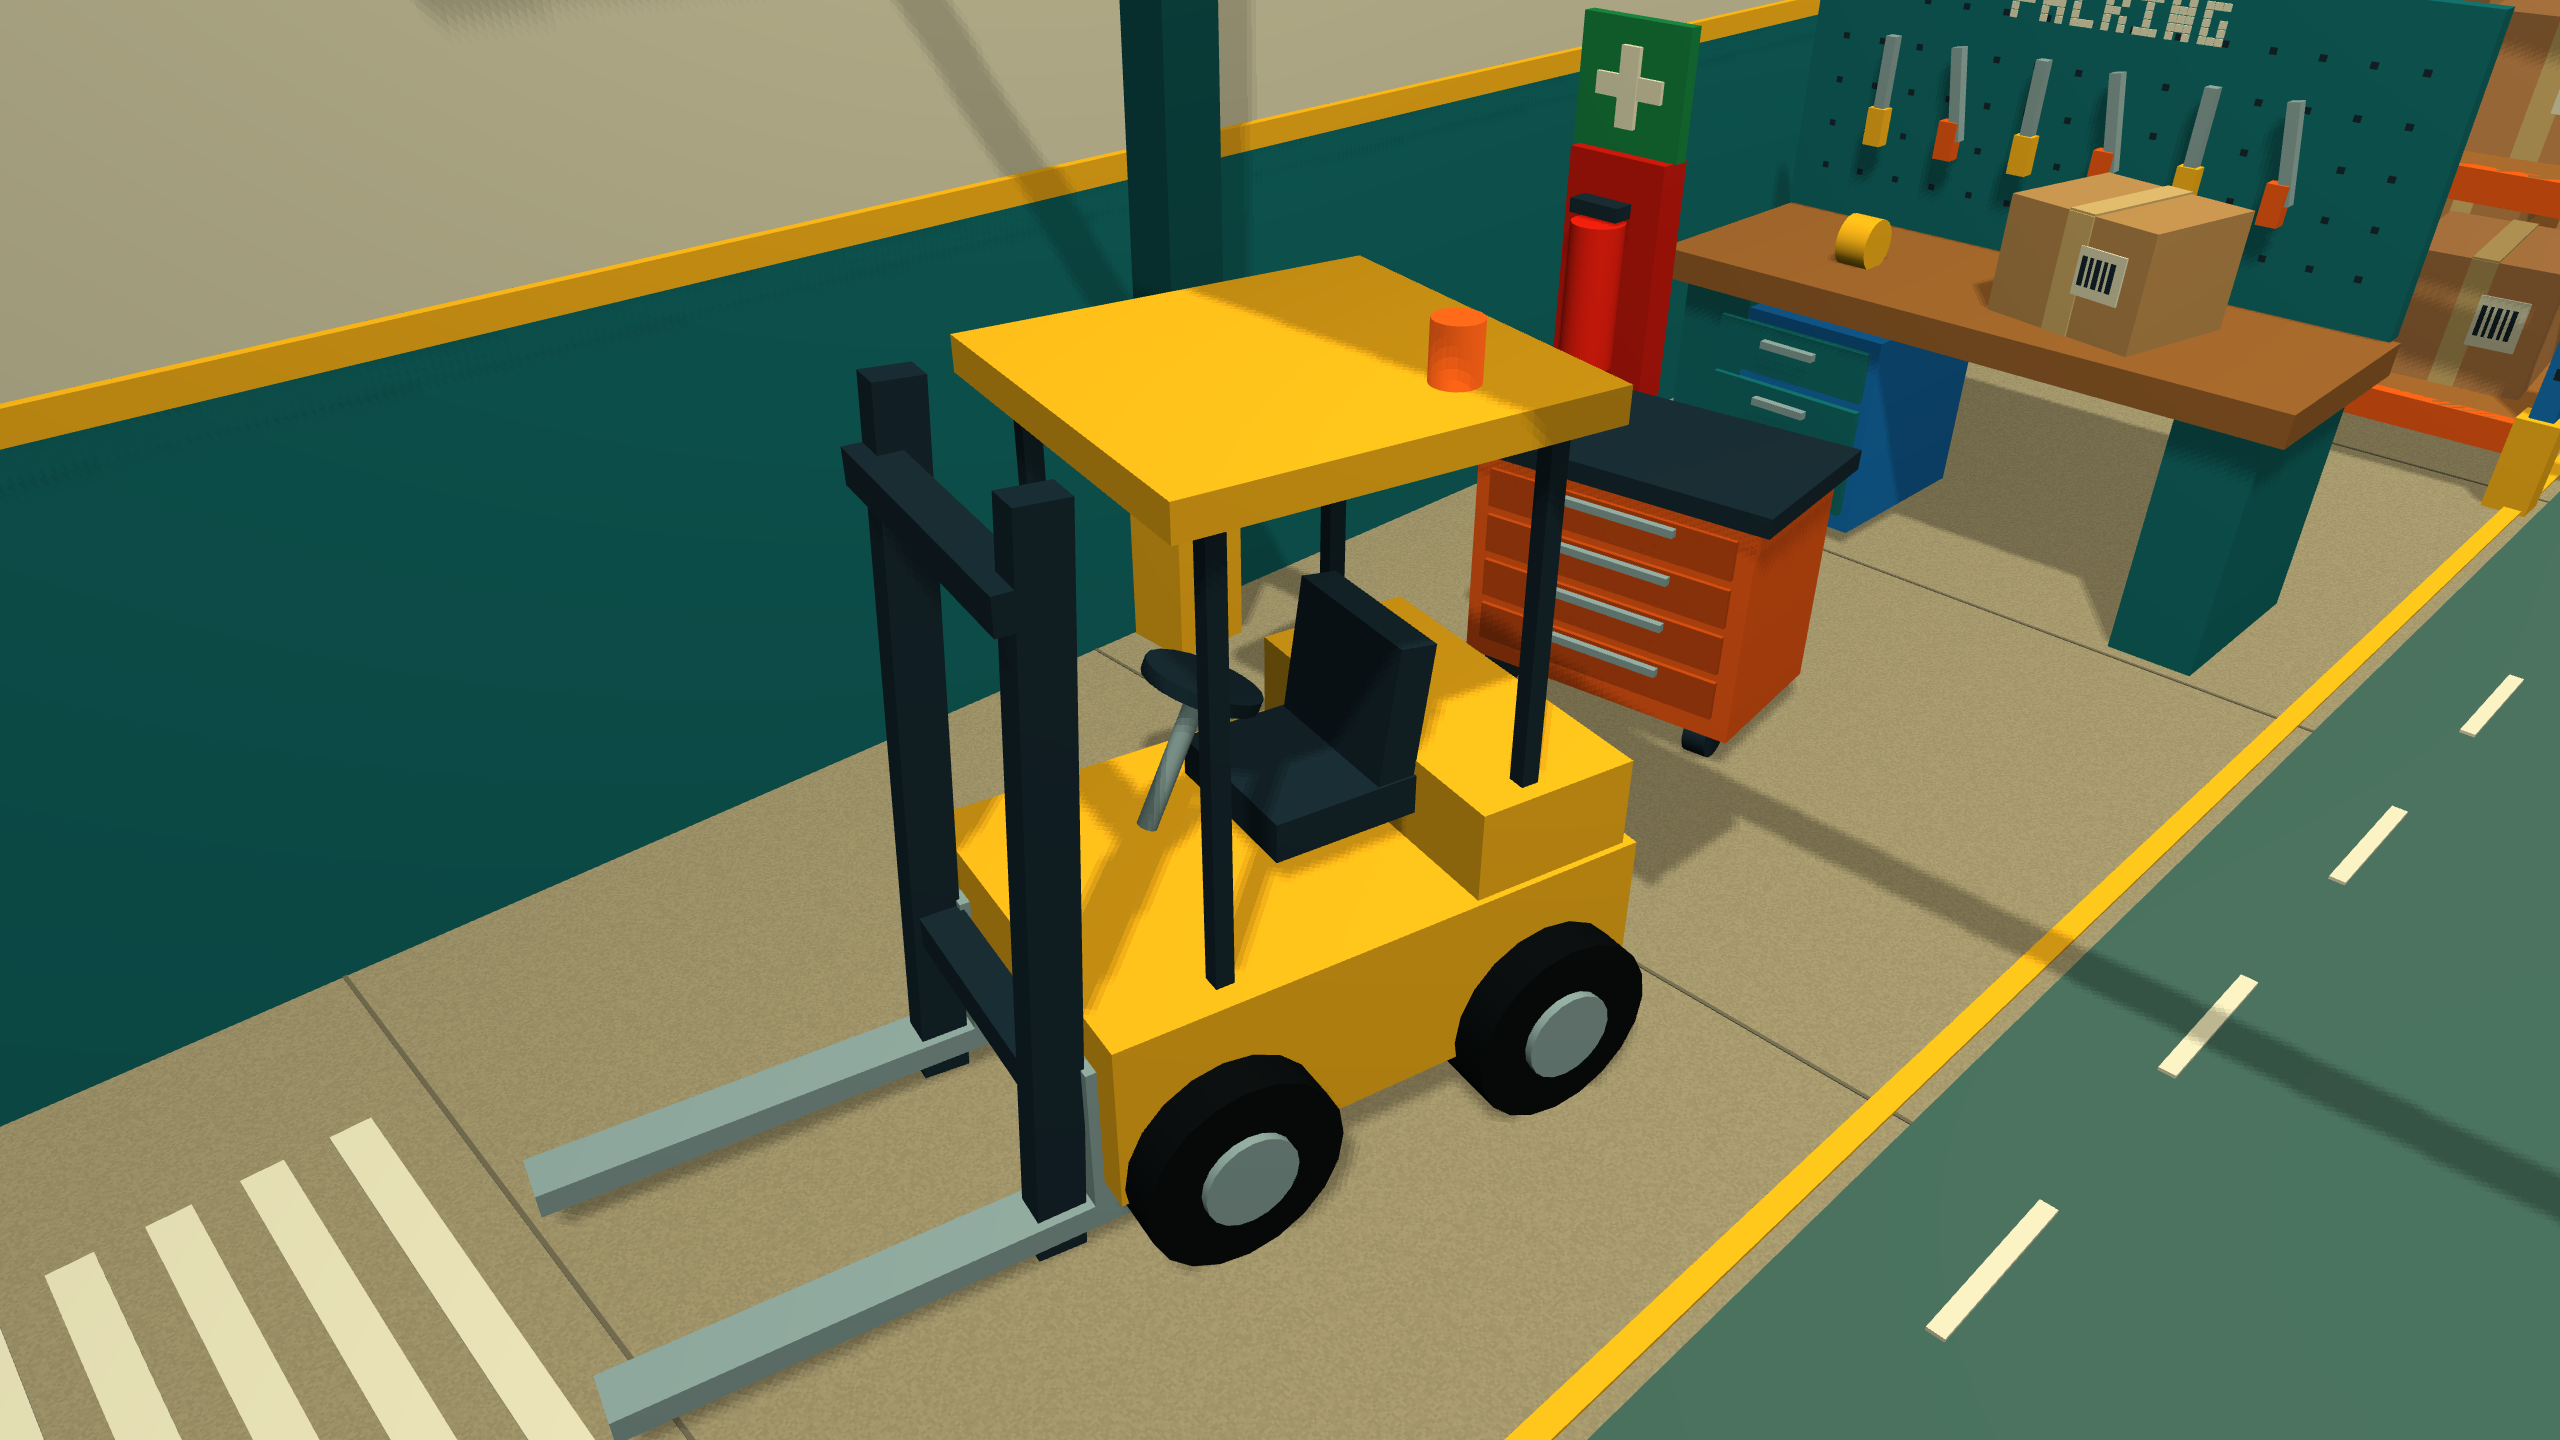
\includegraphics[width=\linewidth]{assets/forklift_crop.png}\par\small\textbf{Forklift:} cube body/forks and cylinder wheels.\end{minipage}\hfill
\begin{minipage}{0.49\linewidth}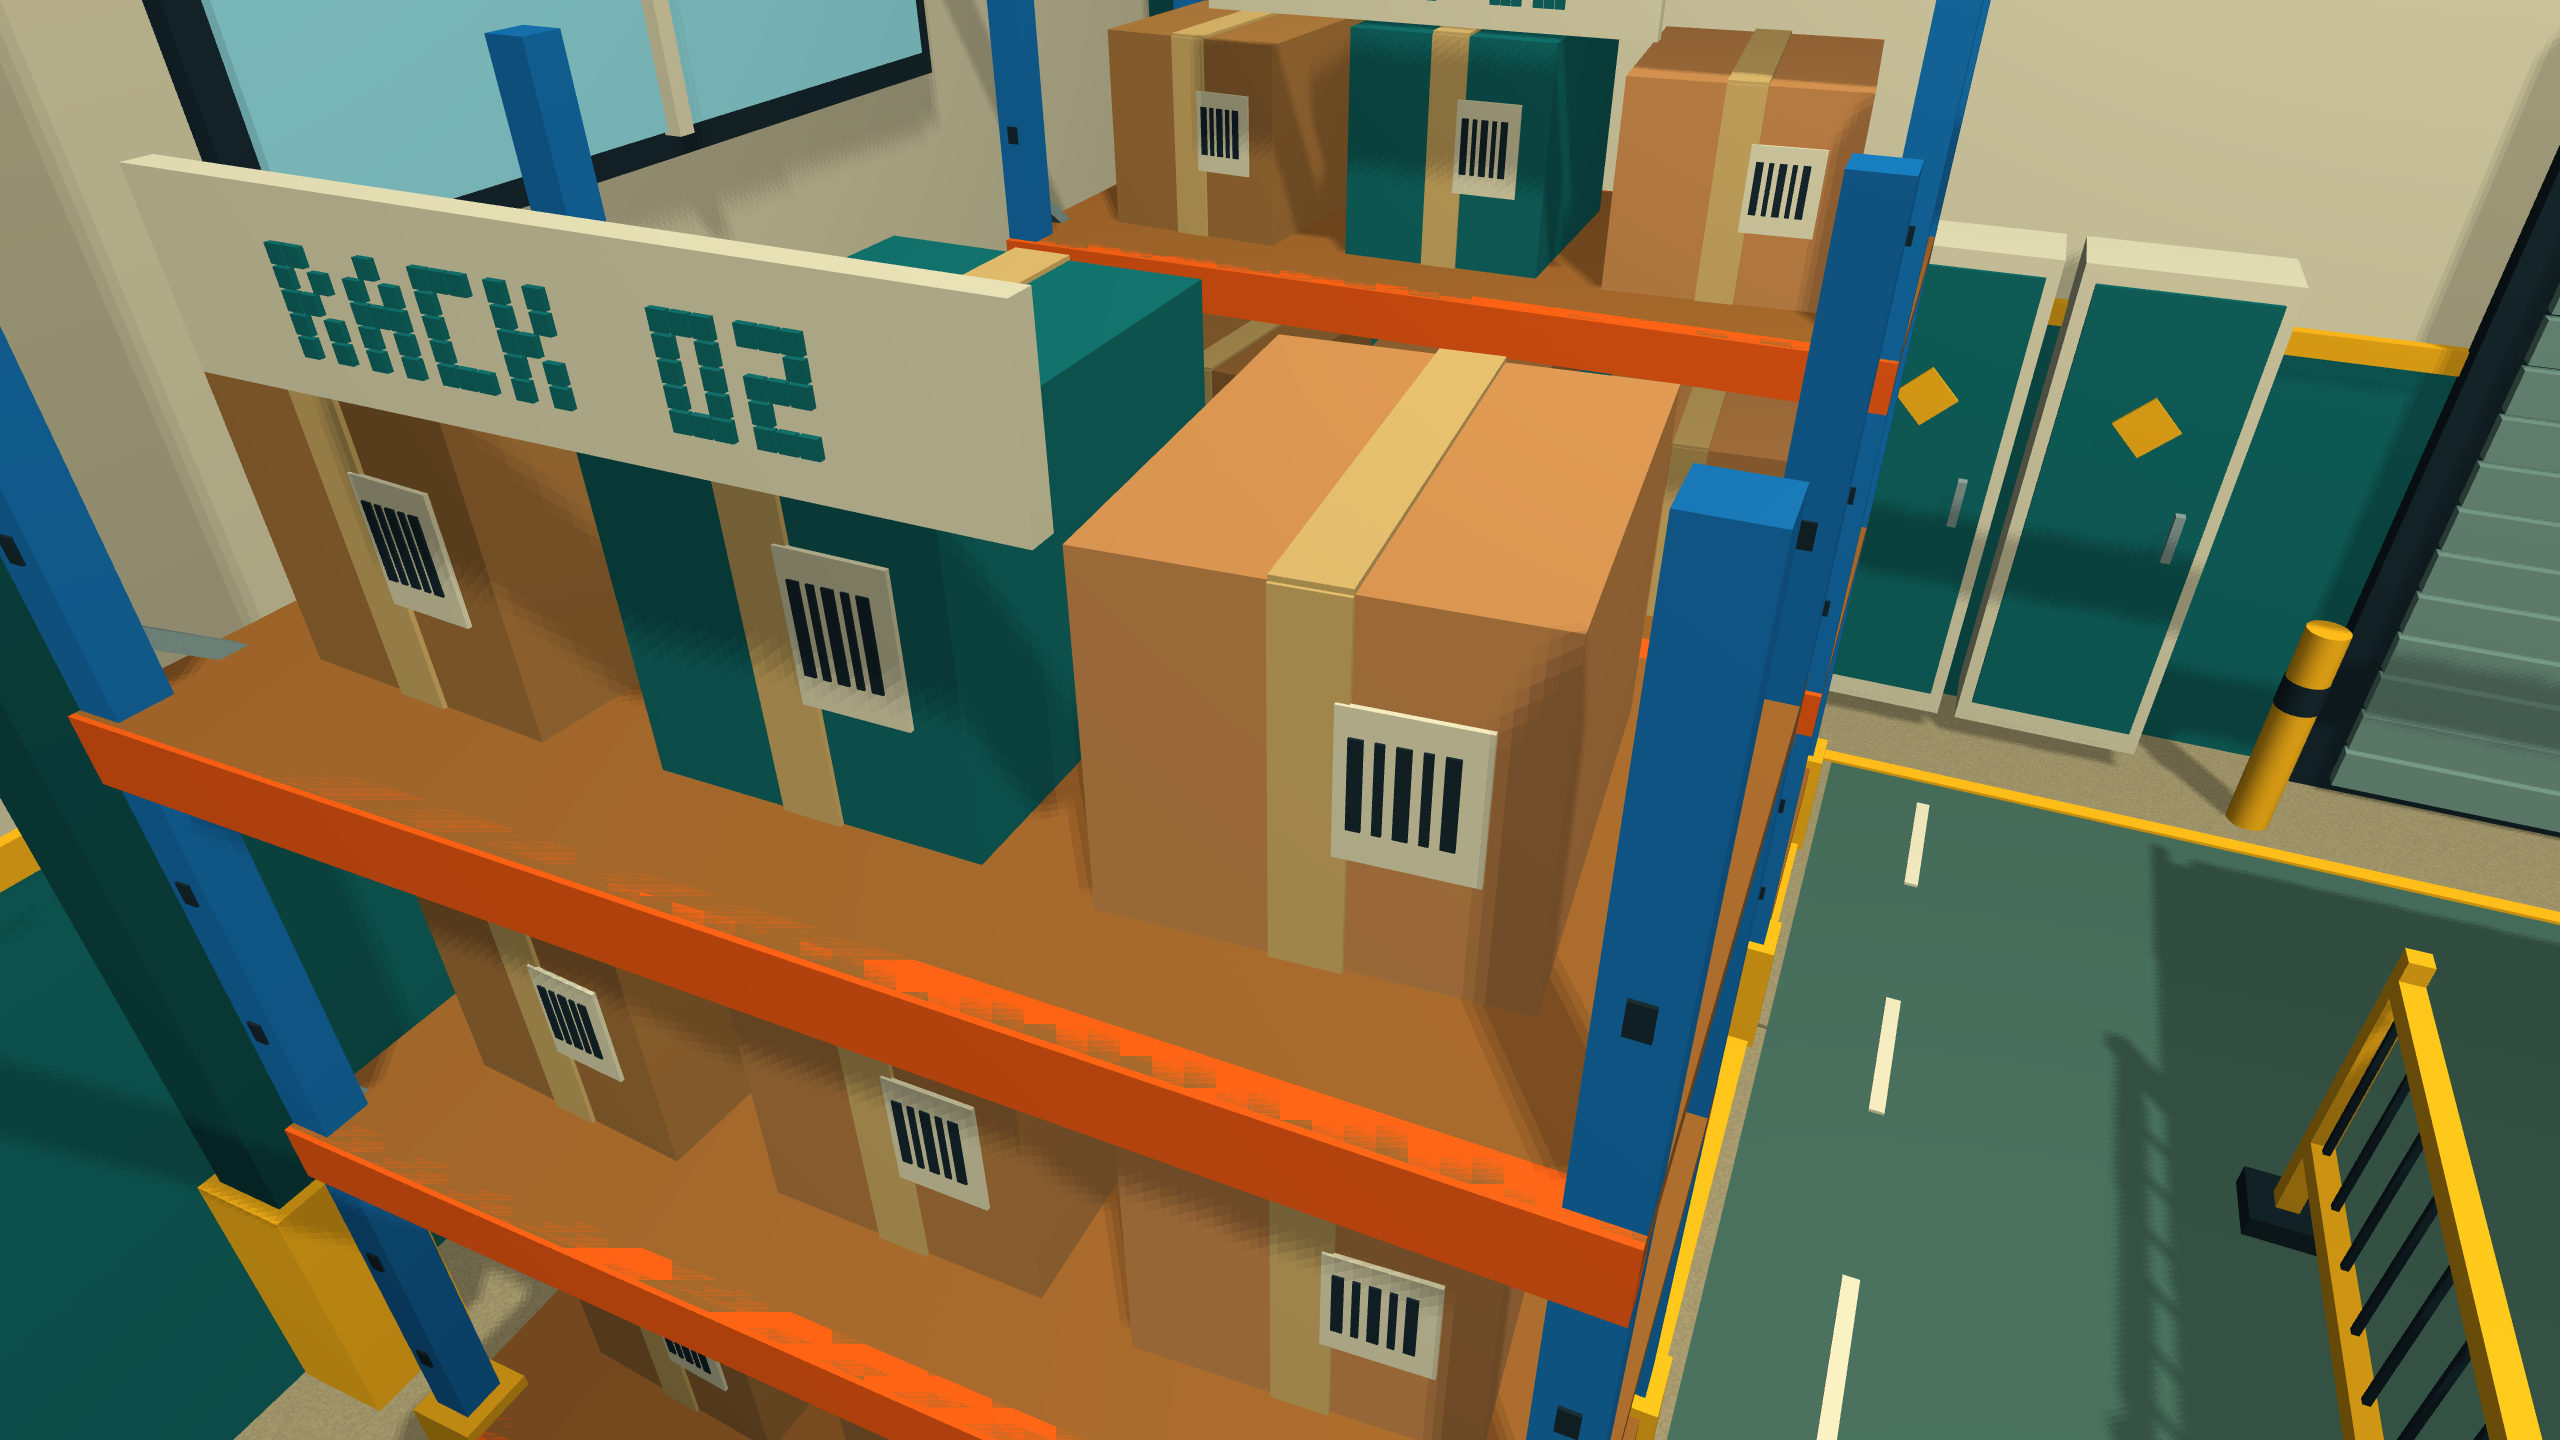
\includegraphics[width=\linewidth]{assets/racks_crop.png}\par\small\textbf{Racks:} repeated posts, shelves and parcels.\end{minipage}
\vspace{3mm}
\begin{minipage}{0.49\linewidth}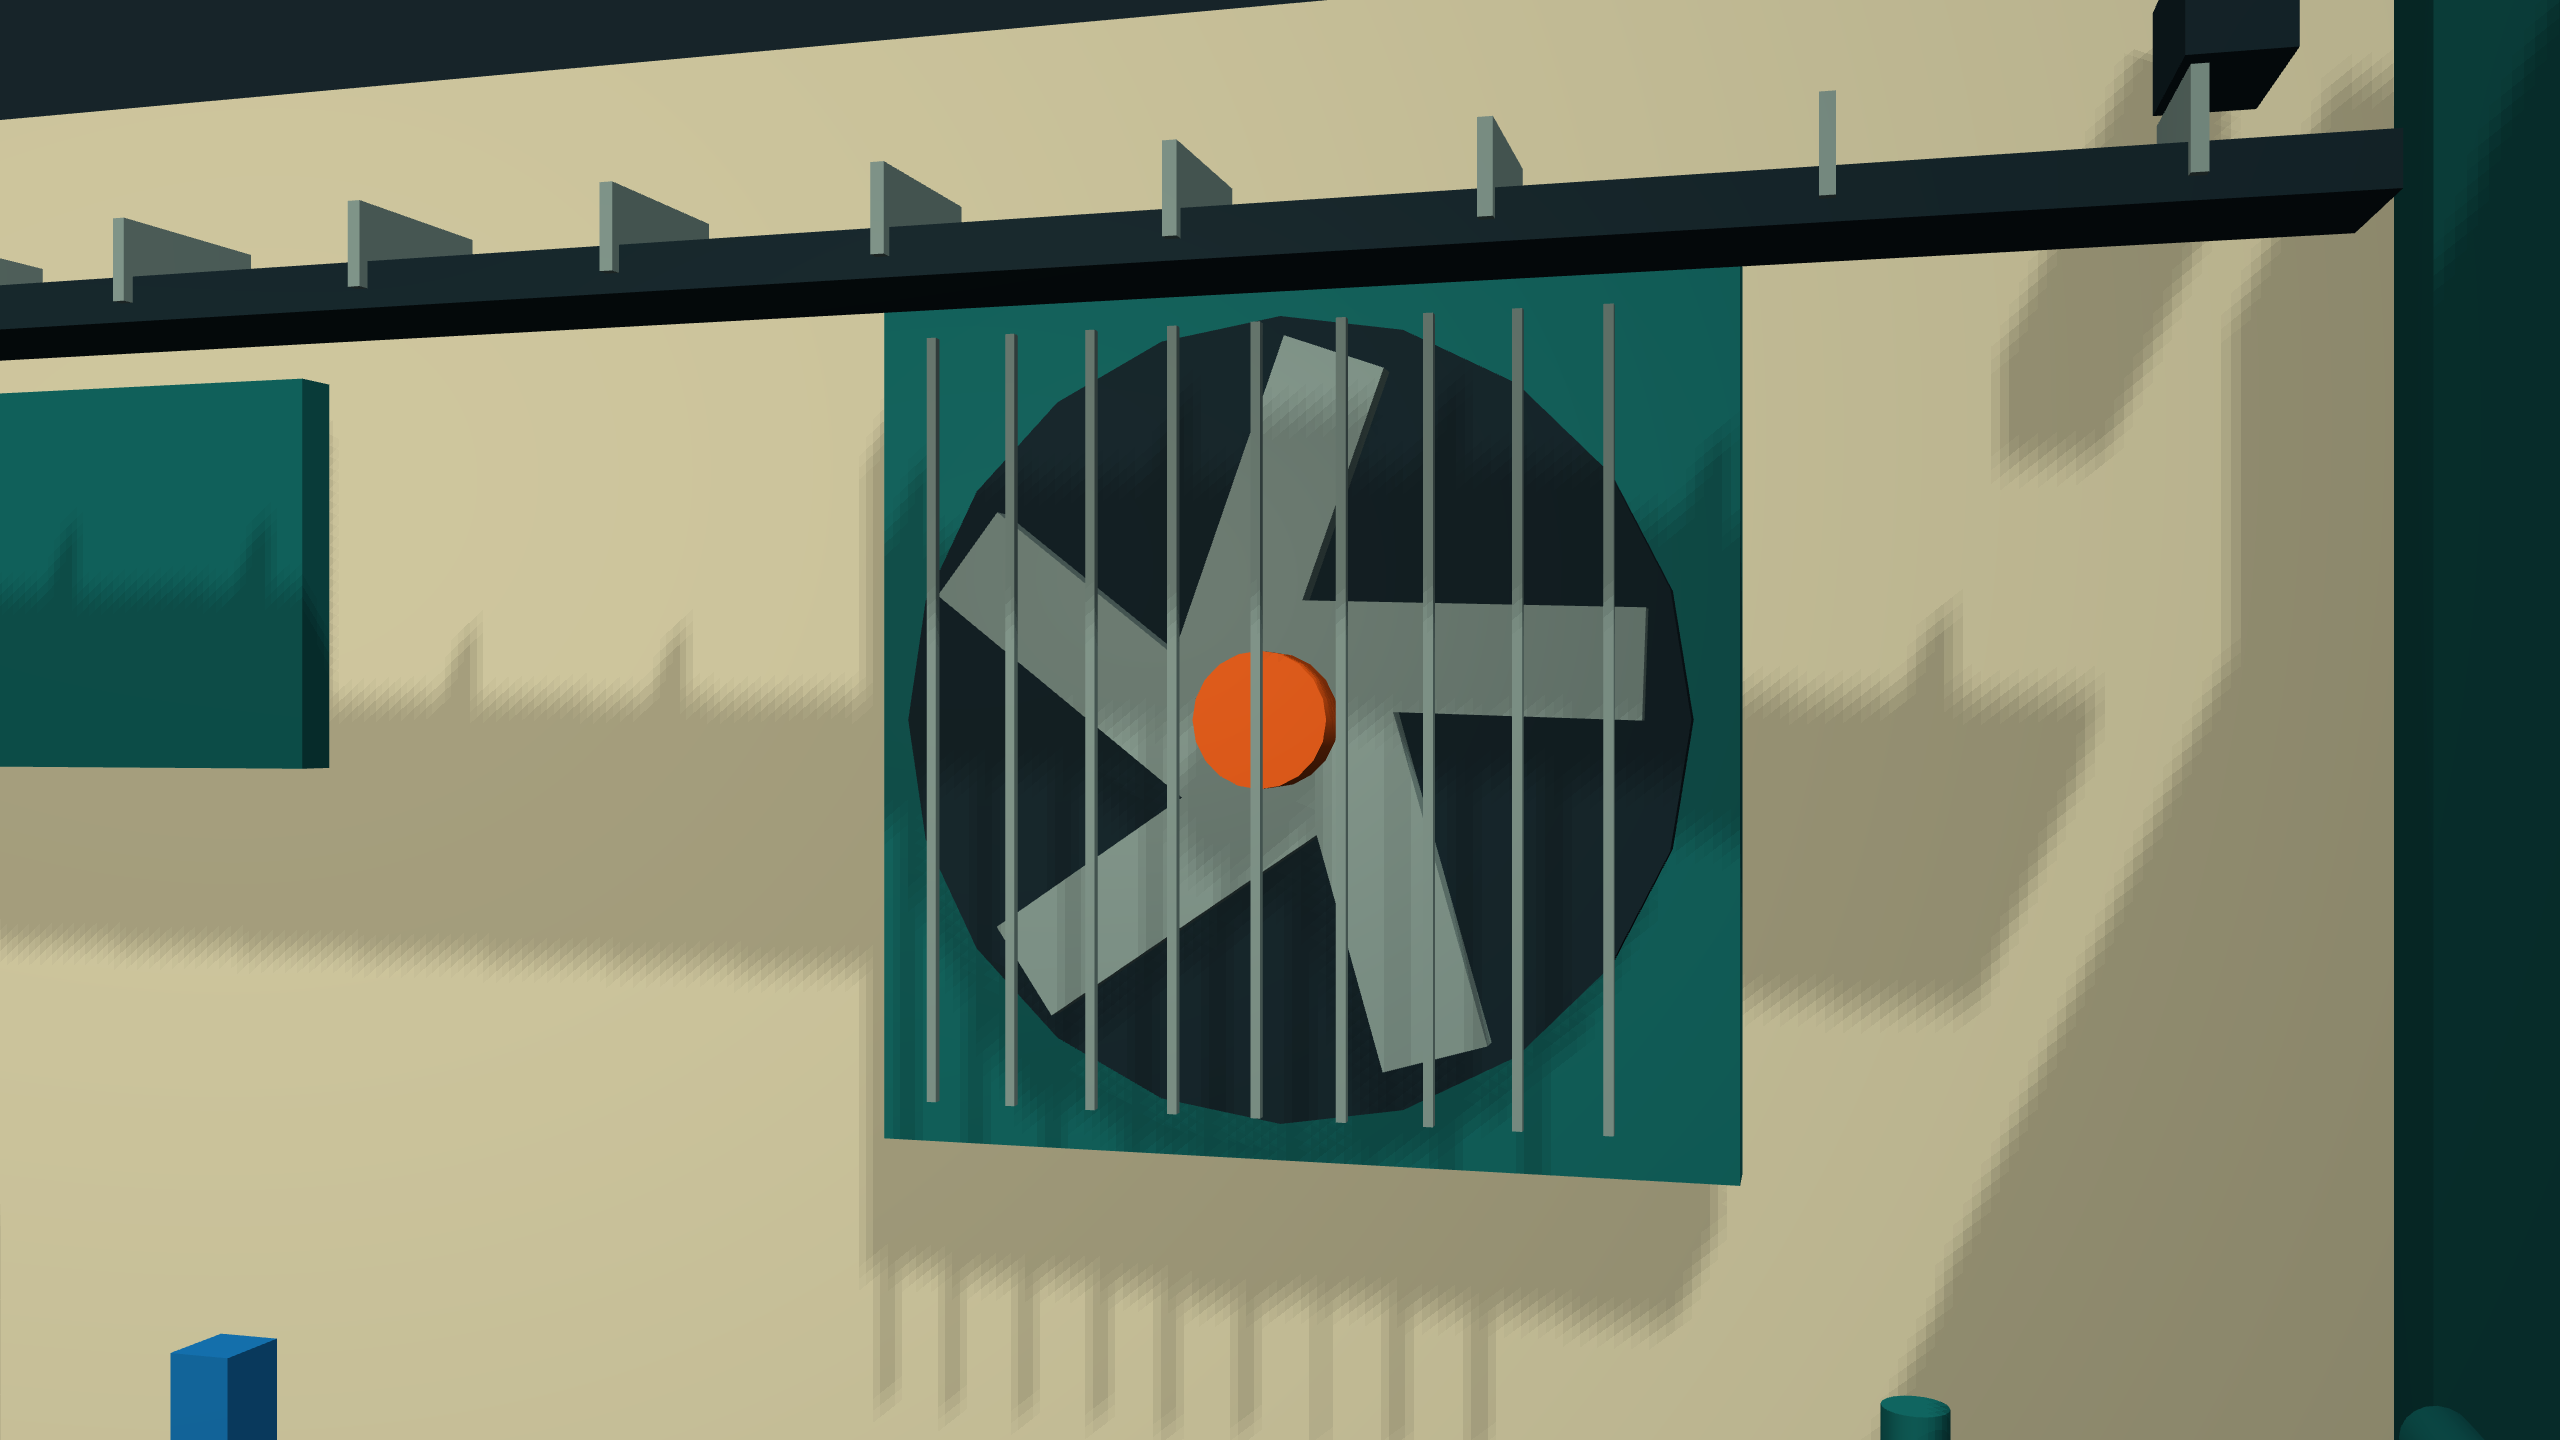
\includegraphics[width=\linewidth]{assets/fan_crop.png}\par\small\textbf{Fan:} five blades rotate around one hub.\end{minipage}\hfill
\begin{minipage}{0.49\linewidth}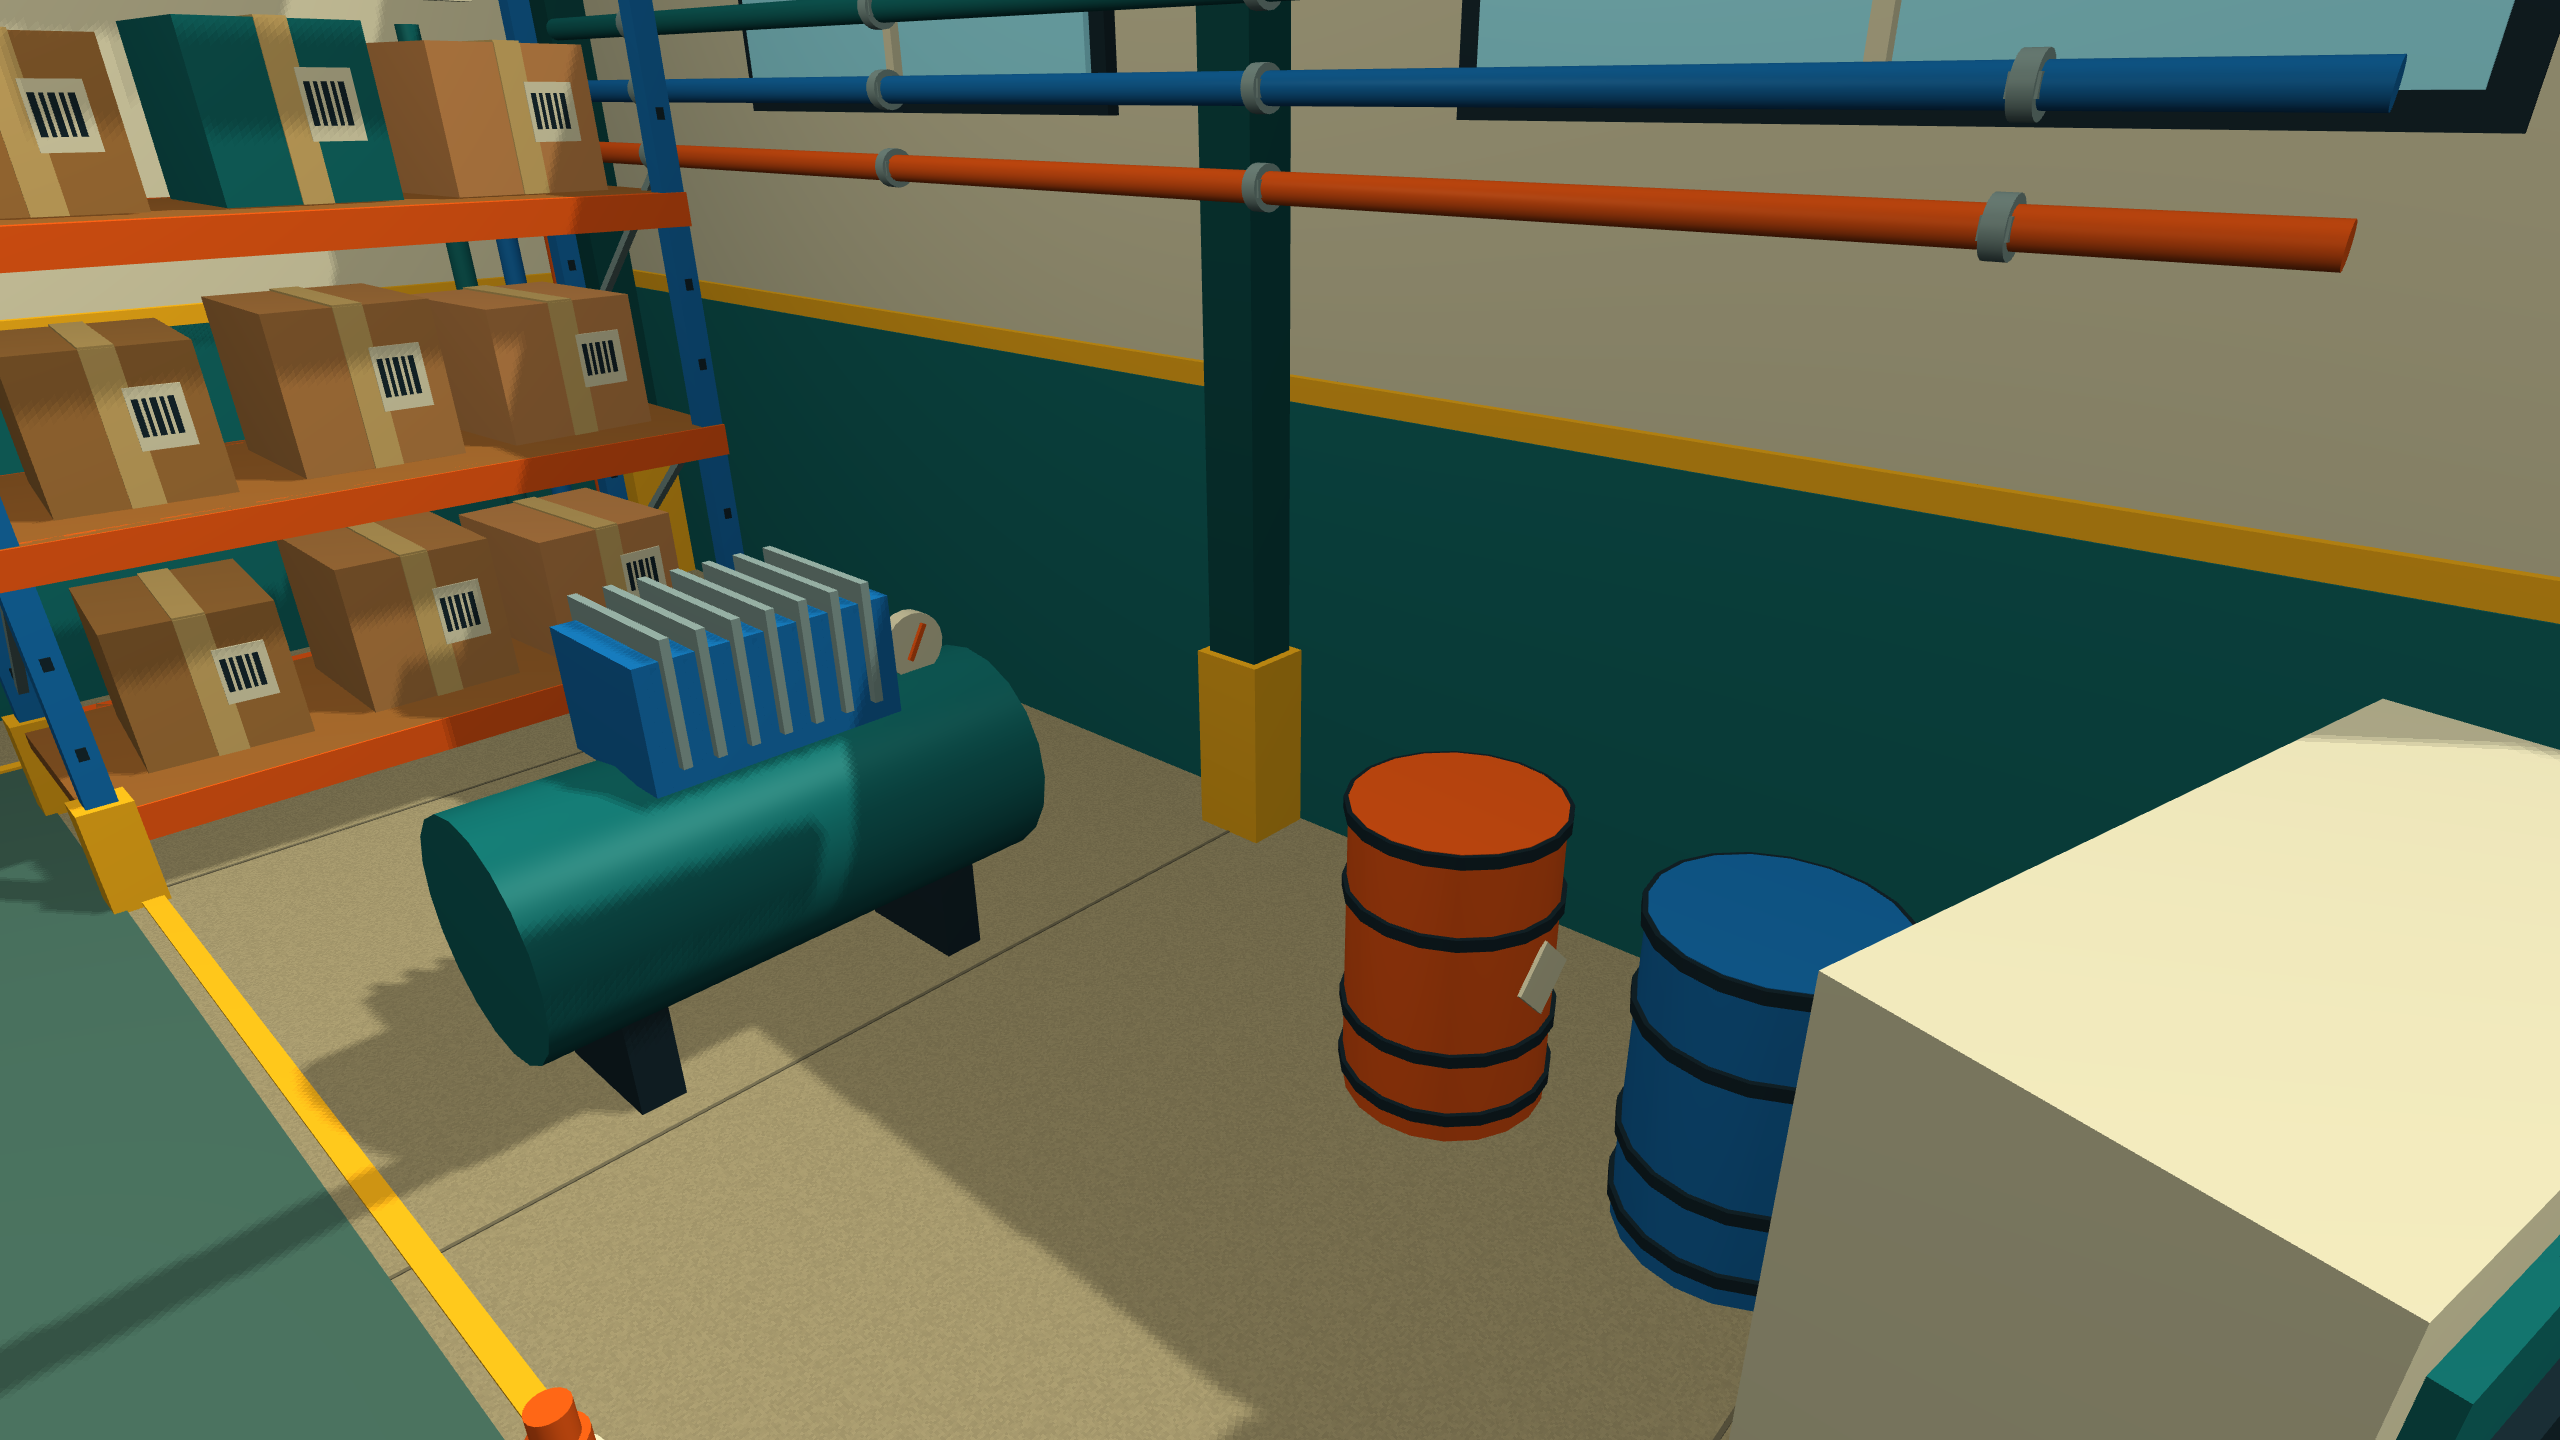
\includegraphics[width=\linewidth]{assets/utilities_crop.png}\par\small\textbf{Utilities:} cylinders form tanks, drums and pipes.\end{minipage}
\caption{Actual close-ups of environment objects. The forklift and utility objects are static; the fan is animated.}
\end{figure}
\subsection{Primitive geometry and hierarchical transforms}
A unit cube has 12 triangles and 36 vertex entries. Scaling it makes belts, legs, shelves and boxes. A 20-segment cylinder has 86 vertex entries and 80 triangles; circular vertices use $x=0.5\cos\theta$, $z=0.5\sin\theta$, $\theta=2\pi i/20$.

The shared helper builds $M=T R_y R_x R_z S$: scale the local shape, rotate it, then place it. Attached parts use $M_{part}=M_{parent}M_{local}$. This keeps labels on boxes and blades around the fan hub. The fan uses $\theta_f'=(\theta_f+150\Delta t)\bmod360$ and keeps turning while sorting is paused.
\par{\small\begin{tabularx}{\textwidth}{@{}L{34mm}Y@{}}\toprule
\textbf{Object} & \textbf{Selected specifications}\\\midrule
Room and floor & $20\times8\times24$ room; floor $(20,0.40,24)$; open front, no solid roof.\\
Racks and loads & Three racks, three shelves each, three cartons per shelf: 27 rack cartons. Three staged pallet loads hold four cartons each.\\
Fan and vehicles & Fan housing diameter 2.12; forklift tyre diameter 0.76; pallet-truck forks length 1.90.\\
Utilities and lettering & Drum diameter 0.90, height 1.38; tank diameter 1.10, length 2.45. Text uses a $3\times5$ cuboid-cell stencil.\\\bottomrule
\end{tabularx}}\par
Normals use $\mathbf{N}=\operatorname{normalize}((M_{3\times3}^{-1})^T\mathbf{n})$, preserving their orientation after non-uniform scaling. The final vertex position is $PVM\mathbf{p}$, using projection, view and model matrices.
\source{\code{Geometry.cpp}: cube/cylinder meshes; \code{FactoryScene.cpp}: transforms, text, environment and fan drawing.}
